\section{Modèle \acs{GPU}}
\subsection{Identification des paramètres}
Les paramètres qui affectent les performances de l'implémentation sur \acs{GPU} sont:
\begin{itemize}
\item le \acs{GPU};
\item la taille du domaine;
\item la taille des blocs;
\item la méthode de transfert;
\item et l'ordre des indices.
\end{itemize}
À l'exception des deux premiers paramètres, les mesures ont montré des configurations optimales pour chacun d'entre eux; à savoir l'utilisation d'une taille de blocs de 32 \textit{threads}, de transferts partiels du domaine et d'adresser la mémoire des populations avec les indices organisés dans l'ordre XYZ.

Ces paramètres n'ont pas besoin d'être inclus dans le modèle de performance, puisqu'ils sont fixés à leur configuration optimale. Seuls le \acs{GPU} utilisé et la taille du domaine simulé sont pris en compte. On considérera également des dimensions optimales pour la taille du domaine (multiples de 32).

\subsection{Formulation du modèle de base} \label{title-modele_performance}

\newcommand{\Time}[0]{T}
\newcommand{\cscoef}[0]{\Psi}
\newcommand{\scoef}[0]{\Gamma}
\newcommand{\rcoef}[0]{\digamma}

%\newcommand{\Time}[0]{T}
%\newcommand{\cscoef}[0]{\omega}
%\newcommand{\scoef}[0]{\tau}
%\newcommand{\rcoef}[0]{\varphi}


Les profilages réalisés en section \ref{title-profilage_gpu} montrent que le temps d'exécution d'une simulation se résume essentiellement à la somme des périodes du \textit{Send}, \textit{Collide \& Stream} et \textit{Receive}. Les mesures suggèrent aussi les tendances, reconnaissable sur chaque type de \acs{GPU}, que suivent leurs courbes en fonction de la taille du domaine.

Pour commencer, la courbe du temps d'exécution de \textit{Collide \& Stream} semble être linéaire. Cette supposition est confirmée par les droites de régression tracées à l'aide des mesures effectuées sur la figure \ref{fig:linear_regr_collide_and_stream}. On peut ainsi exprimer son temps d'exécution $\Time_{cs}$, pour une génération, par la formule suivante, avec $N_x$, $N_y$ et $N_z$ les dimensions du domaine ou $N_{total}$ le nombre total de \textit{lattices} (les itérations) et un coefficient $\cscoef$ déterminé en fonction du \acs{GPU}.
\begin{subequations}
\begin{align}
\Time_{cs} & = \cscoef \cdot N_x \cdot N_y \cdot N_z\\
              & = \cscoef \cdot N_{total} 
\end{align}
\end{subequations}
Ensuite, les courbes du temps d'exécution de \textit{Send} et \textit{Receive} semblent suivre l'évolution de la taille de l'enveloppe transférée (figure \ref{fig:plb_enveloppe_3d}). On exprimera ainsi pour une génération, avec la formule suivante, le temps de transfert $\Time_{send}$  de l'enveloppe extérieur, du \acs{CPU} au \acs{GPU}, réalisé par le \textit{Send}, avec $N_{out}$ la taille de l'enveloppe extérieure et un coefficient $\scoef$ déterminé en fonction du \acs{GPU}.
\begin{subequations}
\begin{align}
\Time_{send} &= \scoef \cdot \Big(N_x \cdot N_y \cdot N_z - (N_x-2)(N_y-2)(N_z-2)\Big)\\
&=  \scoef \cdot N_{out}
\end{align}
\end{subequations}

De la même façon, on exprimera avec la formule suivante, le temps de transfert $\Time_{receive}$ de l'enveloppe intérieur, du \acs{GPU} au \acs{CPU}, réalisé par le \textit{Receive}, avec $N_{in} $ la taille de l'enveloppe intérieure et un coefficient $\rcoef$ déterminé en fonction du \acs{GPU}.
\begin{subequations}
\begin{align}
\Time_{receive} &= \rcoef \cdot \Big((N_x-2)(N_y-2)(N_z-2) - (N_x-4)(N_y-4)(N_z-4)\Big)\\
                     & = \rcoef \cdot N_{in} 
\end{align}
\end{subequations}

Les coefficients $\cscoef \scoef \rcoef$ du modèle de performance, dans sa formulation complète, permettent ainsi d'exprimer le temps d'exécution sur \acs{GPU} pour $g$ générations (itérations) :
\begin{subequations}
\begin{equation}
 \Time_{GPU}  = g  \big( \Time_{cs} + \Time_{send} + \Time_{receive} \big)
\end{equation}
\begin{equation}
\boxed{ \Time_{GPU} = g\big( \cscoef \cdot N_{total} + \scoef \cdot N_{out} + \rcoef \cdot N_{in} \big) }  
\end{equation}
\end{subequations}\\[-\baselineskip]

ou les performances en \acs{LUPS}:
\begin{subequations}
\begin{align}
\acs{LUPS} =  \frac{N_{total} \cdot g}{\Time_{total}}
 \end{align}
\begin{equation}
\boxed{\acs{LUPS} = \frac{N_{total}}{ \cscoef \cdot N_{total} + \scoef \cdot N_{out} + \rcoef \cdot N_{in} }   }  
\end{equation}
\end{subequations}\\[-\baselineskip]

\begin{figure}[h]
	\centering
	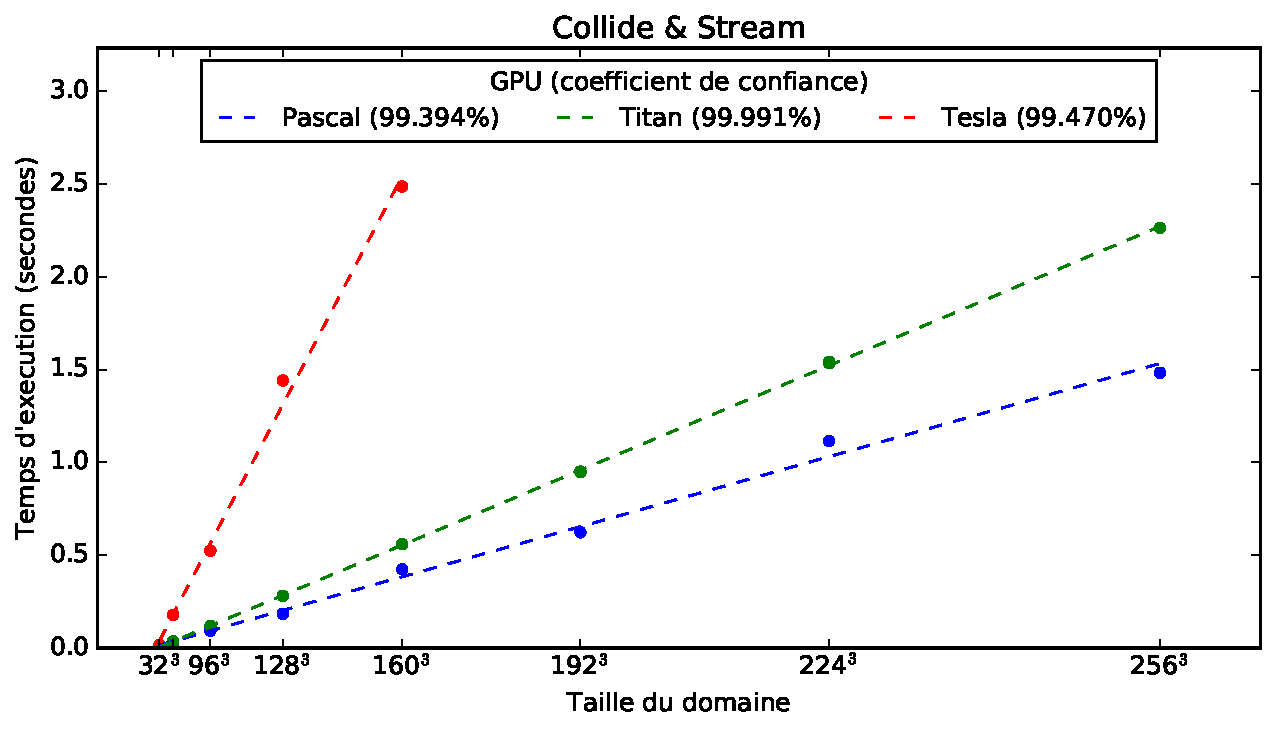
\includegraphics[fbox, scale=0.61]{images/perfs/lbm_simple_lbmcuda/lin_collide_and_stream.pdf}
	\caption{Droite de régression linéaire sur les temps mesurés du \textit{Collide \& Stream}}
	\label{fig:linear_regr_collide_and_stream}
\end{figure}

\subsection{Affinage du modèle }\label{title-affinage_modele_perf}
\subsubsection{Description du modèle de performance pour automate cellulaire}
\citet{albuquerque_performance_2012} propose un modèle de performance pour évaluer le temps d'exécution d'un automate cellulaire sur un \acs{GPU} qu'ils formulent ainsi:
\begin{equation}
\Time_{GPU} = g \cdot \Time_{kernel} = g \bigg( \frac{N_{total}\cdot C_T}{N_{SM}\cdot N_P \cdot D \cdot freq} + \Time_{launch}\bigg)
\end{equation}

avec $N_{SM}$ le nombre de \ac{SM}, $N_P$ le nombre de processeurs sur chaque \ac{SM}, $D$ la profondeur du \textit{pipeline} des processeurs, $freq$ sa fréquence, $C_T$ le travail dont un \textit{thread} est capable et $T_{launch}$ le temps de démarrage d'un kernel.

La formule est aussi étendue pour un \textit{cluster} de \acs{GPU}:
\begin{equation}
\Time_{cluster} = g \bigg( \frac{N_{total}\cdot C_T}{N_{GPU} \cdot N_{SM}\cdot N_P \cdot D \cdot freq} + \Time_{launch}+ \Time_{trans}\bigg)
\end{equation}

avec $N_{GPU}$ le nombre de \acs{GPU} et le temps de transfert $\Time_{trans} = \Time_{lat}+ N_{boundary}/bw$ où $T_{lat}$ est la somme des latences, $N_{boundary}$ les données aux bords à transférer et $bw$ la bande passante. 

Parmi tous ces termes, $N_{SM}$, $N_P$, $D$ et $freq$ sont des propriétés du \acs{GPU} et $C_T$, $\Time_{launch}$, $\Time_{trans}$ sont inféré à partir des simulations.
\subsubsection{Adaptation du modèle}
L'implémentation sur \acs{GPU} de \ac{LBM}, qui est un automate cellulaire, peut profiter de ce modèle pour calculer les coefficients $\cscoef\scoef\rcoef$ formulés en section \ref{title-modele_performance}.  Elle fonctionne comme un \textit{cluster}, en raison des transferts à chaque itération, mais avec $N_{GPU}=1$. On adapte ainsi légèrement le modèle en conséquence:

\begin{equation}
\Time_{GPU} = g \bigg( \frac{N_{total}\cdot C_T}{N_{SM}\cdot N_P \cdot D \cdot freq} + \Time_{launch} + \Time_{trans}\bigg)
\end{equation}

Le coefficient $\cscoef$ qui équivaut au temps requis pour calculer un \textit{lattice} par génération correspond selon ce modèle à l'expression suivante:
\begin{equation}
\cscoef= \frac{C_T}{N_{SM}\cdot N_P \cdot D \cdot freq}
\end{equation}

et s'intègre ainsi à la formule générale:
\begin{equation}
\Time_{GPU} = g \bigg( \cscoef \cdot N_{total} + \Time_{trans} + \Time_{launch}  \bigg)
\end{equation}

Les coefficients  $\scoef$ et $\rcoef$ correspondent au temps requis pour transférer et réorganiser un \textit{lattice}, respectivement vers et depuis le \acs{GPU}. Le modèle définit les temps de transfert avec $\Time_{trans}$.
\begin{equation}
\Time_{trans} = \Time_{lat}+ \frac{N_{boundary}}{bw}
\end{equation}

où $N_{boundary} = N_{out} +  N_{in}$. Les mesures montrent que cette formulation n'est toutefois pas suffisamment précise, car la bande passante est différente d'un sens et dans l'autre. Il faut par conséquent ajuster le modèle pour qu'il utilise un $\Time_{trans}$ différent par type de transfert:
\begin{equation}
\Time_{GPU} = g \bigg( \cscoef \cdot N_{total} + \Time^{send}_{trans} + \Time^{receive}_{trans} + \Time_{launch}  \bigg)
\end{equation}\\[-\baselineskip]

L'implémentation réalisée ne se contente toutefois pas de transférer des données lors du \textit{send} et du \textit{receive}, mais les réorganise sur le \acs{GPU}, dont le kernel a un $C'_T$ différent du premier (on compte par ailleurs 2 $T_{launch}$ supplémentaires).

\begin{equation}
\Time_{GPU} = g \bigg( \cscoef \cdot N_{total} + \Time^{send}_{trans} + \Time^{receive}_{trans} + 2\cdot\frac{N_{boundary}\cdot C'_T}{N_{SM}\cdot N_P \cdot D \cdot freq} + 3\cdot\Time_{launch}  \bigg)
\end{equation}\\[-\baselineskip]

Pour simplifier la lecture, on pose $\phi$, le temps nécessaire à ce kernel pour réorganiser un \textit{lattice}.
\begin{equation}
\Time_{GPU} = g \bigg( \cscoef \cdot N_{total}  + \Time^{send}_{trans} + \Time^{receive}_{trans} + 2\cdot\psi\cdot N_{boundary} + 3\cdot\Time_{launch} \bigg)
\end{equation}\\[-\baselineskip]

\noindent On développe les $T_{trans}$ puis distingue $N_{in}$ et $N_{out}$ des $N_{boundary}$ utilisés jusqu'à présent.
\begin{equation}
\Time_{GPU} = g \bigg( \cscoef \cdot N_{total}  + \frac{N_{out}}{bw_{send}} + \frac{N_{in}}{bw_{receive}} + \psi\cdot (N_{out}+N_{in}) + 3\cdot\Time_{launch} +2\cdot\Time_{lat}\bigg)
\end{equation}\\[-\baselineskip]


On peut ainsi considérer que les coefficients $\scoef$ et $\rcoef$ correspondent aux expressions suivantes, puis les ajouter au modèle.\\

\noindent\begin{minipage}{.5\linewidth}
	\begin{equation}
	\scoef = \frac{1}{bw_{send}} + \psi
	\end{equation}
\end{minipage}%
\begin{minipage}{.5\linewidth}
	\begin{equation}
	\rcoef = \frac{1}{bw_{receive}}  + \psi
	\end{equation}
\end{minipage}\\[\baselineskip]
\begin{equation}
\boxed{\Time_{GPU} = g \bigg( \cscoef \cdot N_{total}  + \scoef \cdot N_{out} + \rcoef \cdot N_{in} + 3\cdot\Time_{launch} +2\cdot\Time_{lat} \bigg)}
\end{equation}\\[-\baselineskip]

En dehors de la formulation détaillée des coefficients $\cscoef\scoef\rcoef$, cette formule est très proche du modèle de base proposé en \ref{title-modele_performance}, à cela qu'il considère $\Time_{launch}$ et $\Time_{lat}$, qu'il faut ajouter à la définition des temps intermédiaires:
\begin{align}
\Time_{cs}           &= \text{\makebox[10pt][c]{$\cscoef$} }\cdot  \text{\makebox[30pt][c]{$N_{total}$} } + \text{\makebox[38pt][c]{$ \Time_{launch}$} } \\
\Time_{send}      &=\text{\makebox[10pt][c]{$\scoef$} }   \cdot   \text{\makebox[30pt][c]{$N_{out}$} }   + \text{\makebox[38pt][c]{$ \Time_{launch}$} }+\Time_{lat} \\
\Time_{receive} &=  \text{\makebox[10pt][c]{$\rcoef$} } \cdot  \text{\makebox[30pt][c]{$N_{in}$} }       + \text{\makebox[38pt][c]{$ \Time_{launch}$} } +\Time_{lat}
\end{align}

\subsection{Calcul et mesure des coefficients $\cscoef\scoef\rcoef$ } \label{title-calcul_coeff}
Le modèle adapté de \cite{albuquerque_performance_2012} en section \ref{title-affinage_modele_perf} nous donne des formules pour calculer les coefficients, à commencer par $\cscoef $.
\begin{equation*}
\cscoef = \frac{C_T}{N_{SM}\cdot N_P \cdot D \cdot freq}
\end{equation*}\\[-\baselineskip]

Les valeurs de $N_{SM}$, $freq$ et $N_{P}$ se trouvent dans la documentation du \acs{GPU} (table \ref{table:gpu_specs}) ou avec Cuda à l'aide de la structure \texttt{cudaDeviceProp}, respectivement dans les champs \texttt{multiProcessorCount}, \texttt{clockRate} et finalement le couple \texttt{major} et \texttt{minor} pour déterminer la \textit{compute capability} du \acs{GPU} et déduire ses $N_{P}$ (table \ref{table:streaming_processeur_per_sm}):

\begin{table}[h]
	\label{table:streaming_processeur_per_sm}
	\renewcommand{\arraystretch}{1.3}
	\centering
	\resizebox{\linewidth}{!}{
		\begin{tabular}{|>{\columncolor{gray!25}}l|c|c|c|c|c|c|c|c|c|c|c|c|c|c|c|}
			\hline
			\rowcolor{gray!25}
			Compute Capability & 1.0 & 1.1 & 1.2 & 1.3 & 2.0 & 2.1 & 3.0 & 3.5 & 3.7 & 5.0 & 5.2 & 6.0& 6.1 & 6.2 \\ 
			\hline 
			Nombre de \acs{SP} & \multicolumn{4}{c|}{8} & 32 & 48 & \multicolumn{3}{c|}{192} & \multicolumn{2}{c|}{128} & 64 & \multicolumn{2}{c|}{128} \\ 
			\hline 
		\end{tabular} 
	}
	\caption{Nombre de \ac{SP} par \acs{SM} \cite{noauthor_cuda_2018}} 
\end{table}

En l'absence d'informations concernant la profondeur $D$ des \textit{pipelines}, le calcul se base sur des valeurs de  $\nicefrac{C_T}{D}$, inférées par les mesures.\\

\noindent\begin{minipage}{.35\linewidth}
	\begin{equation*}
	\bigg(\frac{C_T}{D}\bigg)_{Pascal} = 4773.888
	\end{equation*}
\end{minipage}%
\begin{minipage}{.3\linewidth}
	\begin{equation*}
	\bigg(\frac{C_T}{D}\bigg)_{Titan} = 7407.5904
	\end{equation*}
\end{minipage}
\begin{minipage}{.3\linewidth}
	\begin{equation*}
	\bigg(\frac{C_T}{D}\bigg)_{Tesla} = 4126.72
	\end{equation*}
\end{minipage}\\[\baselineskip]

\noindent On trouve ainsi les valeurs du coefficient $\cscoef$ pour chaque \acs{GPU}:\\

\noindent\begin{minipage}{.33\linewidth}
	\begin{equation*}
	\cscoef_{Pascal} = 0.9 \cdot 10^9
	\end{equation*}
\end{minipage}%
\begin{minipage}{.33\linewidth}
	\begin{equation*}
	\cscoef_{Titan} = 1.35 \cdot 10^9
	\end{equation*}
\end{minipage}
\begin{minipage}{.33\linewidth}
	\begin{equation*}
	\cscoef_{Tesla}  = 6.2 \cdot 10^9
	\end{equation*}
\end{minipage}\\[\baselineskip]

\noindent Les coefficients $\scoef $ et $\rcoef $, dont les valeurs dépendent de toutes les propriétés du modèle, sont plus compliqué à calculer et sont ici inférées par les mesurés: 

\noindent\begin{minipage}{.33\linewidth}
\begin{align*}
\scoef_{Pascal} &= 2.1\cdot 10^{-6}\\
\rcoef_{Pascal} &= 2.25\cdot 10^{-6}\\
\end{align*}
\end{minipage}%
\begin{minipage}{.33\linewidth}
\begin{align*}
\scoef_{Titan} &= 2.1\cdot 10^{-6}\\
\rcoef_{Titan} &= 2.3\cdot 10^{-6}\\
\end{align*}
\end{minipage}%
\begin{minipage}{.33\linewidth}
\begin{align*}
\scoef_{Tesla} &= 9\cdot 10^{-6}\\
\rcoef_{Tesla} &= 7\cdot 10^{-6}\\
\end{align*}
\end{minipage}

\subsection{Courbe théorique}
Par rapport au modèle de base, le modèle affiné introduit les latences $T_{lat}$ et $T_{launch}$. Les mesures de la section \ref{title-latences} montrent que ces valeurs sont de l'ordre de la $[\mu s]$. Elles ont par conséquent une incidence négligeable sur les mesures effectuées où $g=100$.

La figure \ref{fig:courbes_model_perf} illustre les courbes théoriques du modèle de base, tracées avec les coefficients $\cscoef\scoef\rcoef$ définis en section \ref{title-calcul_coeff} et synthétisés dans la table \ref{table:model_perf_coef}. On constate un léger écart entre la courbe du temps total cumulé et les mesures sur Titan. Cet écart correspond au temps restant non qualifié, observé lors des mesures (figure \ref{fig:gpu_rep_times}), et que le modèle ne prend évidemment pas en compte. 

À cette exception près, les courbes suivent fidèlement les temps mesurés. On peut affirmer par conséquent que le modèle de performance fonctionne correctement. 

\begin{table}[H]
	\label{table:model_perf_coef}
	\renewcommand{\arraystretch}{1.3}
	\centering
	\begin{tabular}{|>{\columncolor{gray!25}}l|r|r|r|}
		\hline
		\rowcolor{gray!25}
		\multicolumn{1}{|c|}{} 
		& \multicolumn{1}{c|}{$\cscoef$} 
		& \multicolumn{1}{c|}{$\scoef$} 
		& \multicolumn{1}{c|}{$\rcoef$}\\
		\hline 
		Pascal & $0.9\cdot10^{-9}$ & $2.1\cdot10^{-6}$ & $2.25\cdot10^{-6}$ \\ 
		\hline 
		Titan & $1.35\cdot10^{-9}$ & $2.1\cdot10^{-6}$ & $2.3\cdot10^{-6}$ \\ 
		\hline 
		Tesla & $6.2\cdot10^{-9}$ & $9\cdot10^{-6}$ & $7\cdot10^{-6}$ \\ 
		\hline 
	\end{tabular} 
	\caption{Coefficients $\cscoef\scoef\rcoef$ du modèle de performance}
\end{table}

\begin{figure}[h]
	\centering
	\subfigure[\acs{GPU} Pascal]{%
		\centering
		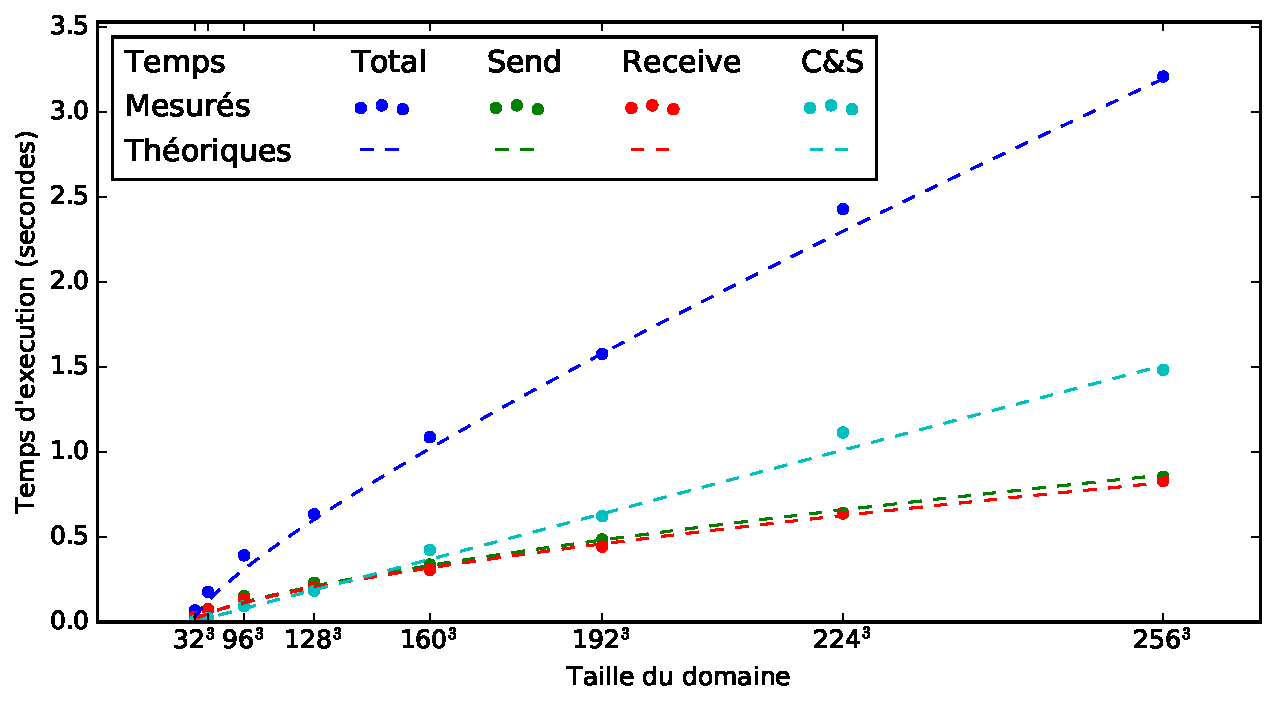
\includegraphics[fbox, scale=0.6]{images/perfs/lbm_simple_lbmcuda/time/perf_model/pascal-opt-64.pdf}
	}
	\subfigure[\acs{GPU} Titan]{%
		\centering
		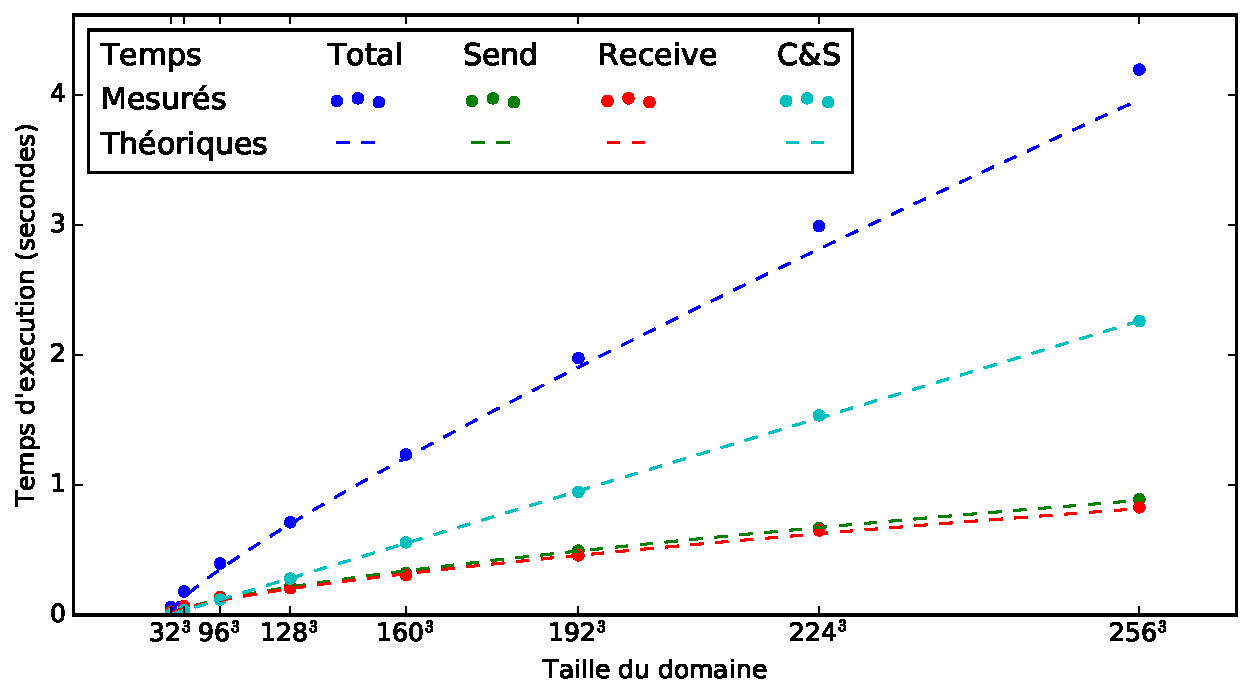
\includegraphics[fbox, scale=0.6]{images/perfs/lbm_simple_lbmcuda/time/perf_model/titan-opt-64.pdf}
	}
	\subfigure[\acs{GPU} Tesla]{%
		\centering
		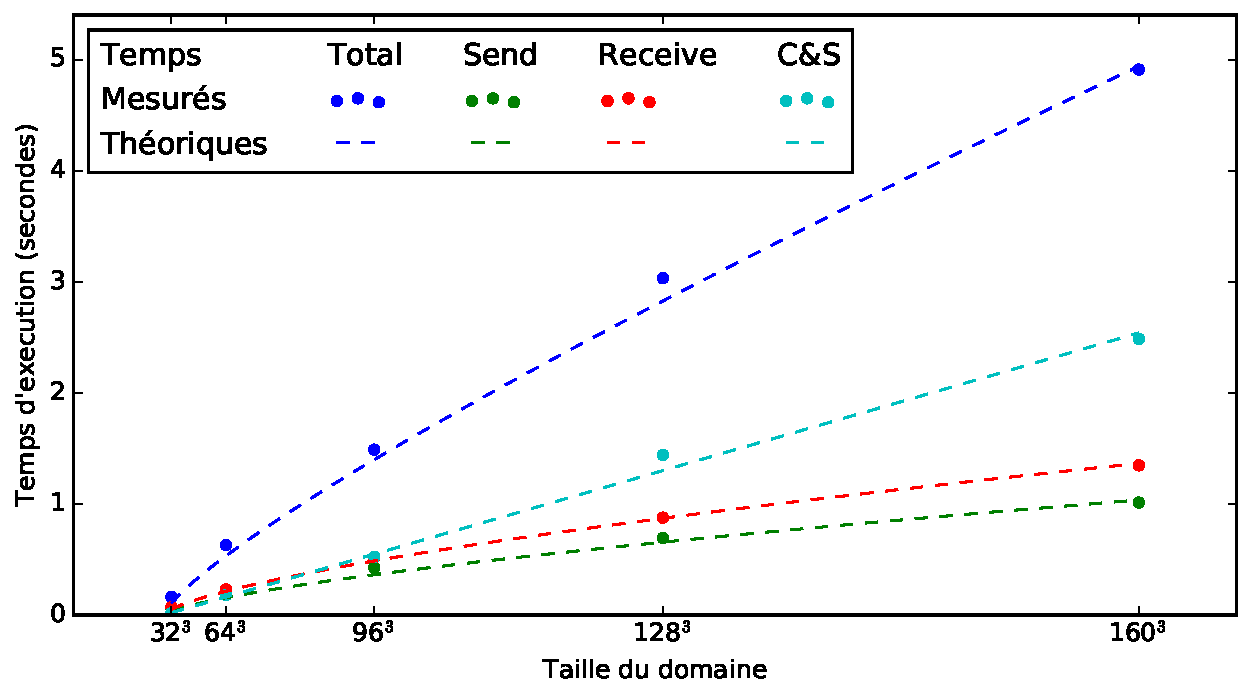
\includegraphics[fbox, scale=0.6]{images/perfs/lbm_simple_lbmcuda/time/perf_model/tesla-opt-64.pdf}
	}
	\caption{Courbes théoriques du modèle de performance}
	\label{fig:courbes_model_perf}
\end{figure}


\section{Modèle hybride}
\subsection{Identification des paramètres}
Les contraintes mémoire, dues à l'implémentation \textit{GPU}, à Palabos et aux machines de test, n'ont pas permis d'obtenir les performances que le système pourrait atteindre dans une configuration optimale. Cette section n'entre par conséquent pas trop en détail dans le modèle de performance hybride, mais esquisse ce à quoi il devrait ressembler. 

L'utilisation de Palabos introduit les paramètres supplémentaires suivants:
\begin{itemize}
\item les dimensions $N_{sx}$, $N_{sy}$ et $N_{sz}$ des sous-domaines (et leur taille $N_{s} = N_{sx}\cdot N_{sy}\cdot N_{sz}$);
\item le nombre $N_{sd}$ de sous-domaines;
\item les paramètres de l'hôte (\acs{CPU}, mémoire, etc.)
\end{itemize}

Les mesures montrent  deux schémas de performances en fonction de la taille d'un sous-domaine. Tandis qu’elles augmentent continuellement sur \acs{GPU}, les performances sur \acs{CPU} restent stables entre 8.5 et 10 \acs{MLUPS} mais baissent jusqu'à moins de 2 \acs{MLUPS} lorsque $N_{sd}$ est petit et ses dimensions petites (forme aplatie).

Ainsi,  la stratégie de découpage du domaine doit trouver un compromis pour la division en sous-domaines pour :
\begin{itemize}
\item maximiser la taille des sous-domaines sur le co-processeur \acs{GPU};
\item en maximiser le nombre pour ceux qui doivent être exécutés sur \acs{CPU};
\item et minimiser le nombre de sous-domaines \acs{CPU} dont aux dimensions trop petites.
\end{itemize}

\noindent Cette question est toutefois le sujet d'un travail différent. Par ailleurs, le modèle esquissé ici ne détaille pas l'impact des paramètres physiques de la machine hôte (fréquence du \acs{CPU}, bande passante, etc.).

\subsection{Formulation du modèle}

Palabos peut s'exécuter sur $N_T$ \textit{threads}. Dans une configuration de calculs séquentiels, avec $N_T=1$, le temps d'exécution total $\Time_{Palabos} $ peut s'exprimer ainsi:
\begin{equation}
\Time_{Palabos} = g \Bigg(\Time_{do} + \sum_{i}^{N_{sd}} \Time_{sd_i} \Bigg) 
\end{equation}\\[-\baselineskip]

avec $\Time_{do}$ le temps d'exécution du \textit{duplicate overlaps} et $\Time_{sd_i}$ le temps calcul du sous-domaine $i$.

Le fonctionnement exact sous-jacent $\Time_{do}$ est caché dans l'implémentation de Palabos. Mais comme les mesures montrent que son temps d'exécution ne varie qu'en fonction de la taille du domaine, on peut alors l'exprimer ainsi:\\

\newcommand{\docoef}[0]{DO}

\begin{equation}
\Time_{do}  = \docoef \cdot N_{Total}
\end{equation}

avec $\docoef$ un coefficient qui correspond au nécessaire au processus de duplication des chevauchements pour s'exécuter sur un \textit{lattice}.

Le temps $\Time_{sd_i}$ dépend du moyen employé pour calculer le sous-domaine. Dans le cas présent, $\Time_{sd_i} = T_{GPU_i}$ \footnote{avec $g_{GPU_i}=1$} du modèle de performance du \acs{GPU}, présenté en section \ref{title-modele_performance} ou \ref{title-affinage_modele_perf}, si c'est le sous-domaine du co-processeur \acs{GPU},  $\Time_{sd_i} = T_{CPU_i}$, le temps de calcul sur \acs{CPU} si c'est un sous-domaine de Palabos.

Lors d'une simulation parallélisée, Palabos distribue à chaque \textit{thread} $t$ les sous-domaines $S_t$ à calculer. Son temps d'exécution $T_{thread_t}$, avec $T_{launch}$ son temps de démarrage, s'exprime ainsi:
\begin{equation}
\Time_{thread_t} =  \Time_{launch} + \sum_{s\in S} T_{sd_s} 
\end{equation}\\[-\baselineskip]

Finalement, le temps d'exécution $\Time_{Palabos}$ s'exprime ainsi:

\begin{equation}
\Time_{Palabos} =   g \Bigg(\Time_{do} + \max{(T_{thread}}) \Bigg)
\end{equation}\\[-\baselineskip]

avec $\forall t$,  $\max{(T_{thread}}) \ge T_{thread_t}$. En effet, les \textit{threads} dont l'exécution est terminée doivent attendre les autres pour recevoir les bordures de leur voisin afin de calculer la génération suivante. Il est par conséquent primordial de diviser le domaine correctement pour réduire au maximum l'attente entre chaque \textit{thread} pour ne pas gaspiller de temps de calcul potentiel.